\subsection*{1. Uso da chamada de sistema fork}
\addcontentsline{toc}{section}{1. Uso da chamada de sistema fork}

\subsubsection{1.1 - Compile e execute o programa prog1.c. Explique o seu funcionamento, detalhando o uso das chamadas de sistema usadas.}
\addcontentsline{toc}{subsection}{Exercício 1.1}

\vspace{-0.5em}
\begin{minipage}{\textwidth}
  \hspace{-1em}
  \centering
  \lstinputlisting[language=C]{pratica1/prog1.c}
  \captionof{figure}{Código fonte do programa prog1.c}
  \label{prog1}
  \hspace{1em}
\end{minipage}
\vspace{0.5em}

Na linha 11, o comando \textbf{fork()} cria um processo filho idêntico ao pai a menos de seu identificador. Nas linhas 13 e 19 o código faz a diferenciação do programa baseado em seu identificador, assim, ``criando'' códigos diferentes pros diferentes processos. Utiliza-se o processo com PID 0 para o processo filho, fora da convenção de usar o processo 0 como pai. Na linha 16 o processo somente aguarda por 10 segundos antes de ser finalizado. Na linha 23 o processo espera pelo processo 0, o processo filho, e imprime seu status.

\vspace{2em}
\begin{minipage}{\textwidth}
    \hspace{-1em}
    \centering
    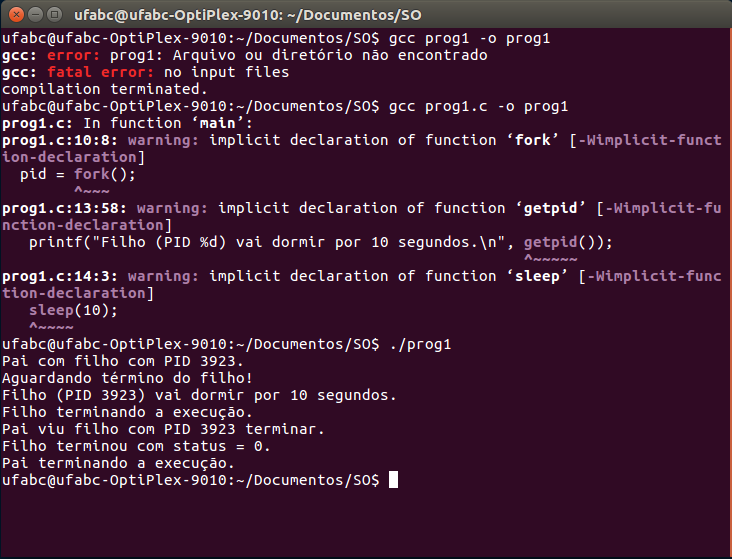
\includegraphics[scale=.4]{pratica1/prog1.png}
    \captionof{figure}{Execução do código prog1.c}
    \label{prog1png}
    \hspace{1em}
\end{minipage}
\vspace{0.5em}

\subsubsection{1.2 - Envie o sinal SIGINT ao processo fillho: kill -SIGINT PID, em que PID é o PID do processo filho mostrado na tela. O que aconteceu nesse caso? Justifique.}
\addcontentsline{toc}{subsection}{Exercício 1.2}

\vspace{2em}
\begin{minipage}{\textwidth}
    \hspace{-1em}
    \centering
    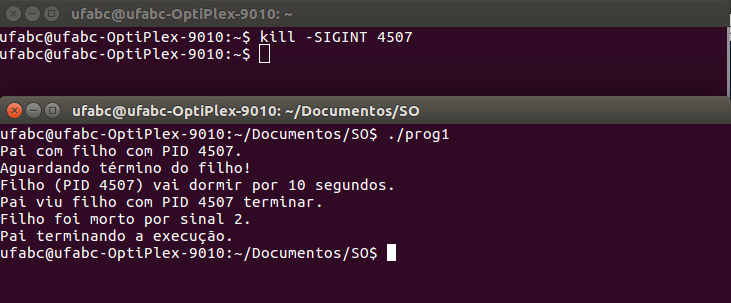
\includegraphics[scale=.4]{pratica1/prog1kill.png}
    \captionof{figure}{Execução do código prog1.c interrompido por um sinal}
    \label{prog1killpng}
    \hspace{1em}
\end{minipage}
\vspace{0.5em}

O sinal enviado para o processo filho foi o SIGINT, sinal de interrupção, conforme o manual do linux, cujo tratamento padrão é o término do processo.

\vspace{2em}
\begin{minipage}{\textwidth}
    \hspace{-1em}
    \centering
    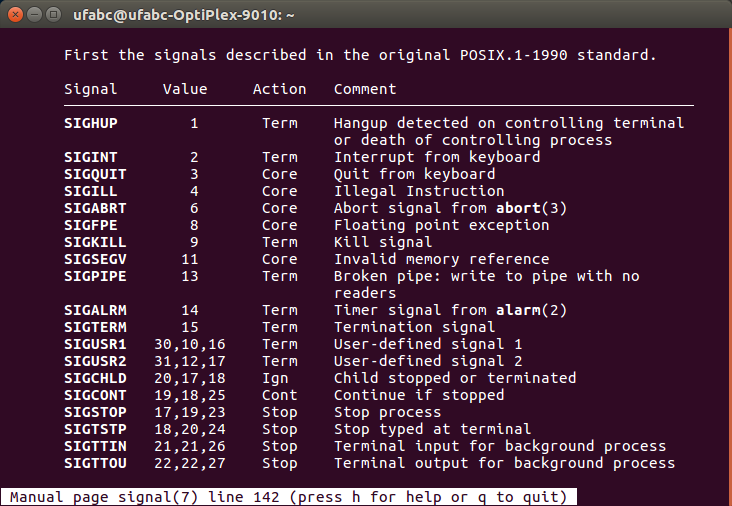
\includegraphics[scale=.4]{pratica1/signals.png}
    \captionof{figure}{Trecho do manual do Linux sobre sinais}
    \label{signals}
    \hspace{1em}
\end{minipage}
\vspace{0.5em}

\subsection*{2. Sinais como condição de erro.}
\addcontentsline{toc}{section}{2. Sinais como condição de erro.}

\subsubsection{2.1 - Compile e execute o programa prog2.c. Por que o processo filho é terminado?}
\addcontentsline{toc}{subsection}{Exercício 2.1}

\vspace{-0.5em}
\begin{minipage}{\textwidth}
  \hspace{-1em}
  \centering
  \lstinputlisting[language=C]{pratica1/prog2.c}
  \captionof{figure}{Código fonte do programa prog2.c}
  \label{prog2}
  \hspace{1em}
\end{minipage}
\vspace{0.5em}

Ao executar a linha 15, ocorre um erro aritmético e então o sinal 8 é enviado ao filho, e, consultando a figura \ref{signals}, vemos que corresponde ao sinal SIGFPE, erro de ponto flutuante, cujo tratamento padrão é encerrar o programa e realizar o ``dump core'' - despejo de memória.

\vspace{2em}
\begin{minipage}{\textwidth}
    \hspace{-1em}
    \centering
    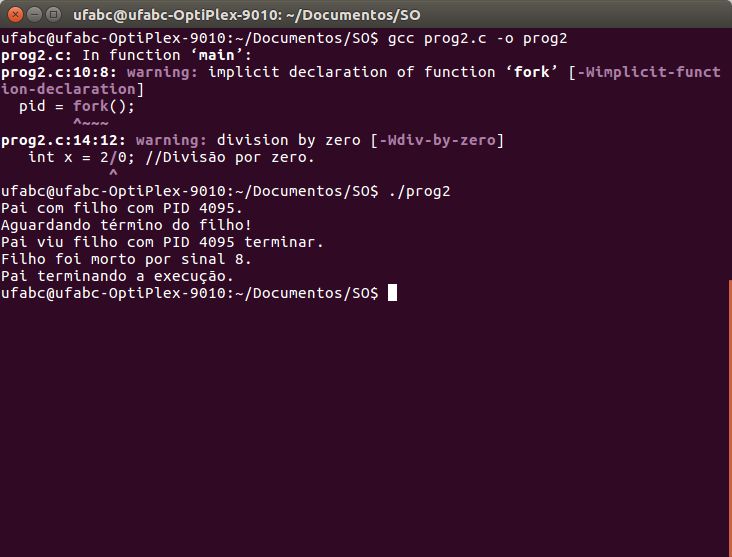
\includegraphics[trim=0 250 0 0,clip,scale=.4]{pratica1/prog2.png}
    \captionof{figure}{Execução do código prog2.c}
    \label{prog2png}
    \hspace{1em}
\end{minipage}
\vspace{0.5em}

\subsubsection{2.2 - Compile e execute o programa prog3.c. Por que o processo filho é terminado?}
\addcontentsline{toc}{subsection}{Exercício 2.2}

\vspace{-0.5em}
\begin{minipage}{\textwidth}
  \hspace{-1em}
  \centering
  \lstinputlisting[language=C]{pratica1/prog3.c}
  \captionof{figure}{Código fonte do programa prog3.c}
  \label{prog3}
  \hspace{1em}
\end{minipage}
\vspace{0.5em}

Ao executar a linha 15, ocorre uma referência a um endereço inválido na memória e então o sinal 11 é enviado ao filho, e, consultando a figura \ref{signals}, vemos que corresponde ao sinal SIGSEGV, referência de memória inválida, cujo tratamento padrão também é encerrar o programa e realizar o ``dump core'' - despejo de memória.

\vspace{2em}
\begin{minipage}{\textwidth}
    \hspace{-1em}
    \centering
    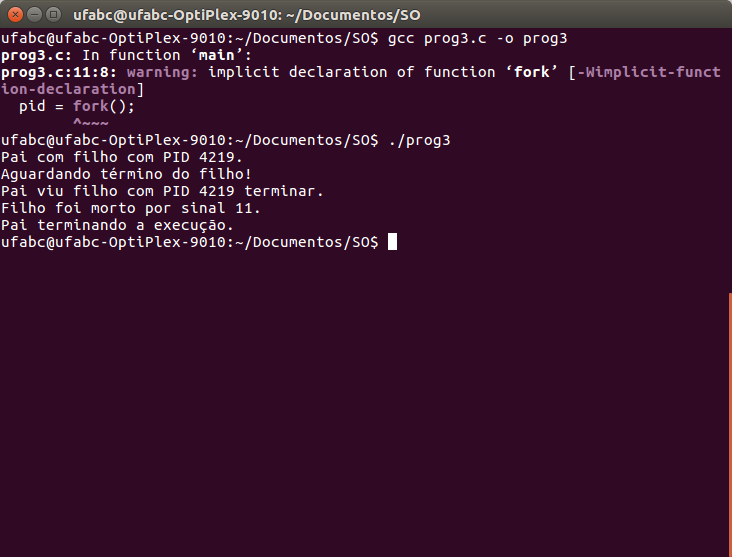
\includegraphics[trim=0 300 0 0,clip,scale=.4]{pratica1/prog3.png}
    \captionof{figure}{Execução do código prog3.c}
    \label{prog3png}
    \hspace{1em}
\end{minipage}
\vspace{0.5em}

\subsection*{3. Como tratar um sinal?}
\addcontentsline{toc}{section}{3. Como tratar um sinal?}

\subsubsection{3.1 - Compile e execute o programa prog4.c. Em um segunda execução, envie o sinal SIGINT ao processo fillho. Compare as duas execuções e comente. O que é necessário fazer para tratar um sinal?}
\addcontentsline{toc}{subsection}{Exercício 3.1}

\vspace{-0.5em}
\begin{minipage}{\textwidth}
  \hspace{-1em}
  \centering
  \lstinputlisting[language=C]{pratica1/prog4.c}
  \captionof{figure}{Código fonte do programa prog4.c}
  \label{prog4}
  \hspace{1em}
\end{minipage}
\vspace{0.5em}

É necessário o comando signal, que passa um tratador de sinais para o sistema, para um sinal em específico.

\vspace{2em}
\begin{minipage}{\textwidth}
    \hspace{-1em}
    \centering
    \begin{minipage}[b]{0.49\textwidth}
        \centering
        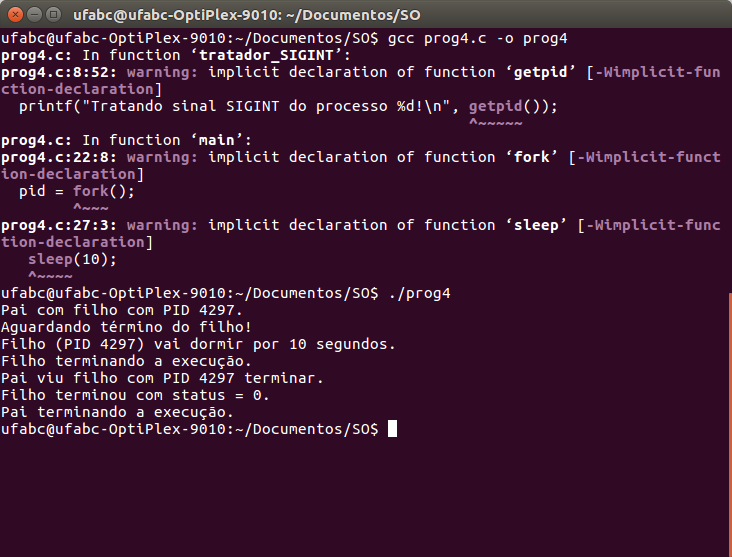
\includegraphics[trim=0 110 0 0,clip,scale=.3]{pratica1/prog4.png}
        \captionof{figure}{Execução do código prog4.c}
        \label{prog4png}
    \end{minipage}
    \hfill
    \begin{minipage}[b]{0.49\textwidth}
        \centering
        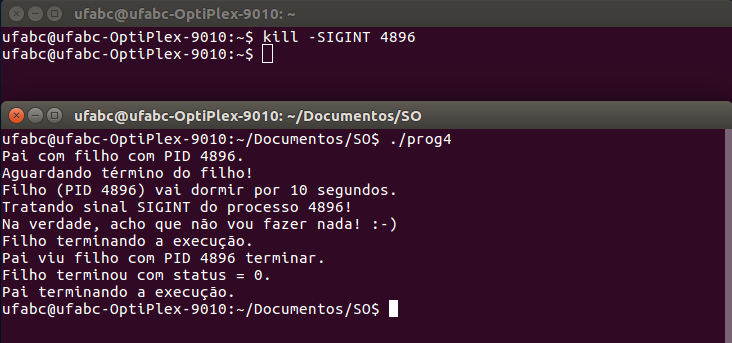
\includegraphics[scale=.3]{pratica1/prog4kill.png}
        \captionof{figure}{Interrupção do código prog4.c}
        \label{prog4killpng}
    \end{minipage}
    \hspace{1em}
\end{minipage}

\subsubsection{3.2 - Modifique o programa prog4.c para tratar a condição de erro do programa prog3.c. Foi possível tratar o sinal e continuar a execução? Justifique.}
\addcontentsline{toc}{subsection}{Exercício 3.2}

\vspace{-0.5em}
\begin{minipage}{\textwidth}
  \hspace{-1em}
  \centering
  \lstinputlisting[language=C]{pratica1/prog4mod.c}
  \captionof{figure}{Código fonte do programa prog4.c modificado}
  \label{prog4mod}
  \hspace{1em}
\end{minipage}
\vspace{0.5em}

Mesmo instalando um tratador de sinais para o sinal SIGSEGV, este sinal não admite tratamento, e é novamente lançado pelo sistema, então nosso tratador executa infinitamente.

\vspace{2em}
\begin{minipage}{\textwidth}
    \hspace{-1em}
    \centering
    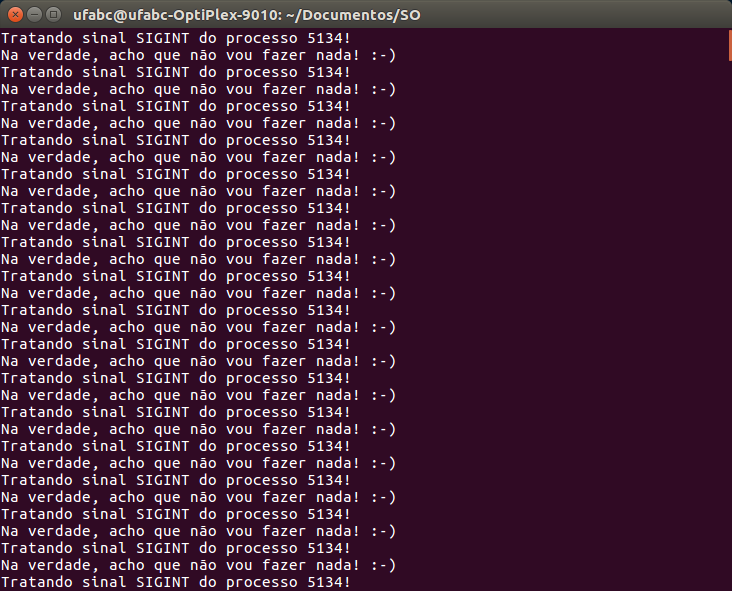
\includegraphics[scale=.4]{pratica1/prog4mod.png}
    \captionof{figure}{Execução infinita do código prog4.c modificado}
    \label{prog4modpng}
    \hspace{1em}
\end{minipage}

\subsection*{4. Como mascarar um sinal?}
\addcontentsline{toc}{section}{4. Como mascarar um sinal?}

\subsubsection{4.1 -  Compile e execute o programa prog5.c. Durante sua execução, envie o sinal SIGQUIT ao processo filho. Em um segunda execução, envie o sinal SIGTERM ao processo filho. Compare as duas execuções e comente. O que é necessário fazer para mascarar um sinal? }
\addcontentsline{toc}{subsection}{Exercício 4.1}

\vspace{-0.5em}
\begin{minipage}{\textwidth}
  \hspace{-1em}
  \centering
  \lstinputlisting[language=C]{pratica1/prog5.c}
  \captionof{figure}{Código fonte do programa prog5.c}
  \label{prog5}
  \hspace{1em}
\end{minipage}
\vspace{0.5em}

É necessário instalar uma máscara, definindo um conjunto de sinais a serem bloqueados. No prog5, isso é feito nas linhas 23 a 25, onde a máscara bloqueia somente o sinal SIGQUIT. Quando executado, o programa efetivamente bloqueia o recebimento do sinal SIGQUIT, mas não do SIGTERM que não foi definido na máscara, assim o processo é encerrado por este último sinal. 

\vspace{2em}
\begin{minipage}{\textwidth}
    \hspace{-1em}
    \centering
    \begin{minipage}[b]{0.49\textwidth}
        \centering
        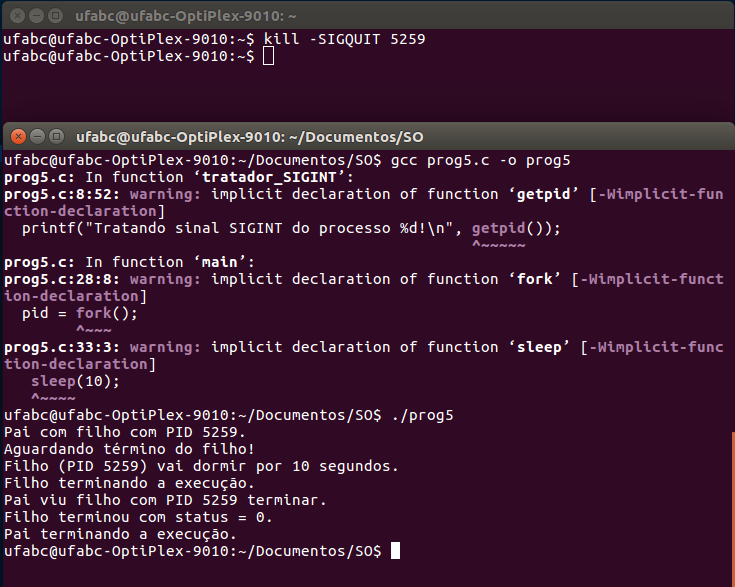
\includegraphics[scale=.3]{pratica1/prog5kill1.png}
        \captionof{figure}{Primeira interrupção do código prog5.c}
        \label{prog5kill1png}
    \end{minipage}
    \hfill
    \begin{minipage}[b]{0.49\textwidth}
        \centering
        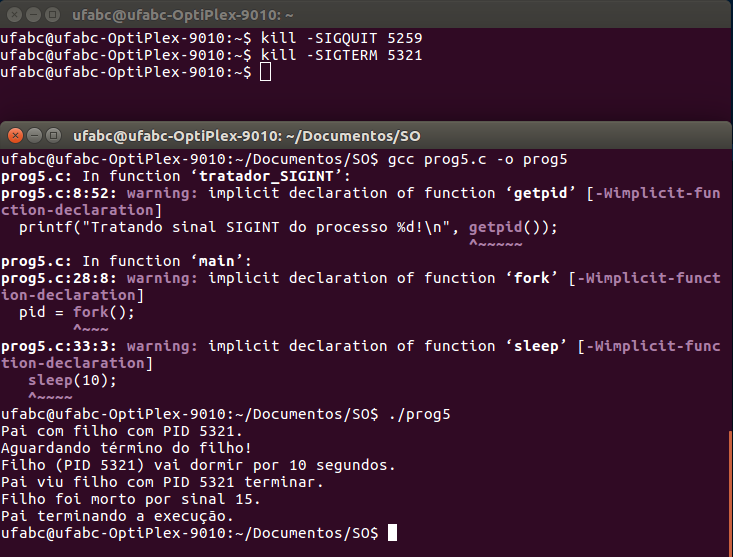
\includegraphics[scale=.3]{pratica1/prog5kill2.png}
        \captionof{figure}{Segunda interrupção do código prog5.c}
        \label{prog5kill2png}
    \end{minipage}
    \hspace{1em}
\end{minipage}

\subsubsection{4.2 - É possível tratar ou mascarar o sinal SIGKILL ou SIGSTOP? Justifique}
\addcontentsline{toc}{subsection}{Exercício 4.2}

Não, esses sinais sequer chegam a ser tratados pelo processo, já que o sistema operacional consome este sinal e respectivamente encerra ou pausa o processo alvo, conforme o manual do linux.

\vspace{2em}
\begin{minipage}{\textwidth}
    \hspace{-1em}
    \centering
    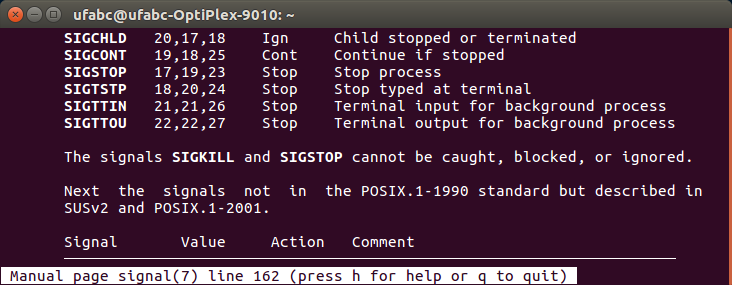
\includegraphics[trim=0 0 0 0,clip,scale=.4]{pratica1/sigkill.png}
    \captionof{figure}{Manual do linux sobre os sinais SIGKILL e  SIGSTOP}
    \label{prog4modpng}
    \hspace{1em}
\end{minipage}

\subsection*{5. Criação de threads}
\addcontentsline{toc}{section}{5. Criação de threads}

\subsubsection{5.1 - Compile com a opção -pthread o programa prog6.c. Execute-o várias vezes e comente sobre as saídas. Explique o funcionamento do programa.}
\addcontentsline{toc}{subsection}{Exercício 5.1}

\vspace{-0.5em}
\begin{minipage}{\textwidth}
  \hspace{-1em}
  \centering
  \lstinputlisting[language=C]{pratica1/prog6.c}
  \captionof{figure}{Código fonte do programa prog6.c}
  \label{prog4mod}
  \hspace{1em}
\end{minipage}
\vspace{0.5em}

O programa cria threads sequencialmente e as faz imprimir seu identificador. No entanto, a saída é completamente desordenada e imprevisível, pois cada thread depende da liberação do dispositivo de saída e do escalonamento do processo operacional.

\vspace{2em}
\begin{minipage}{\textwidth}
    \hspace{-1em}
    \centering
    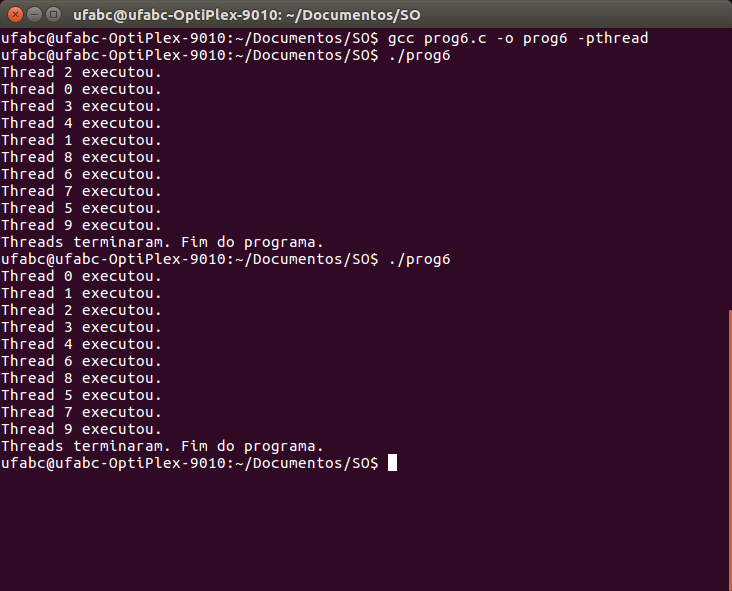
\includegraphics[trim=0 110 0 0,clip,scale=.4]{pratica1/prog6.png}
    \captionof{figure}{Execução do código prog6.c}
    \label{prog4modpng}
    \hspace{1em}
\end{minipage}

\subsubsection{5.2 - Compile com a opção -pthread o programa prog7.c. Execute-o várias vezes e comente sobre as saídas. Qual a solução para o problema apresentado?}
\addcontentsline{toc}{subsection}{Exercício 5.2}

\vspace{-0.5em}
\begin{minipage}{\textwidth}
  \hspace{-1em}
  \centering
  \lstinputlisting[language=C]{pratica1/prog7.c}
  \captionof{figure}{Código fonte do programa prog7.c}
  \label{prog4mod}
  \hspace{1em}
\end{minipage}
\vspace{0.5em}

O programa cria duas threads para acessar uma variável compartilhada, simplesmente alterando seu valor e imprimindo. No entanto, ao contrário do que se esperava, as threads não imprimem o mesmo valor que alteram. Isso porque um escalonamento da thread pode ocorrer entre a atribuição e a impressão da variável, e ela está sujeita a ser alterada pela outra thread antes de ser impressa. Isso configura uma região crítica, onde se espera que os comandos sejam imediatamente executados na ordem declarada sem intercalamento (dentro de um mesmo programa, não dá para evitar por exemplo interrupções pelo sistema operacional). Para solucionar, é necessário um uso de semáforos para que a outra thread não opere a variável mesmo quando capaz, quando o escalonamento ocorrer, até que a thread anterior permita.

\vspace{2em}
\begin{minipage}{\textwidth}
    \hspace{-1em}
    \centering
    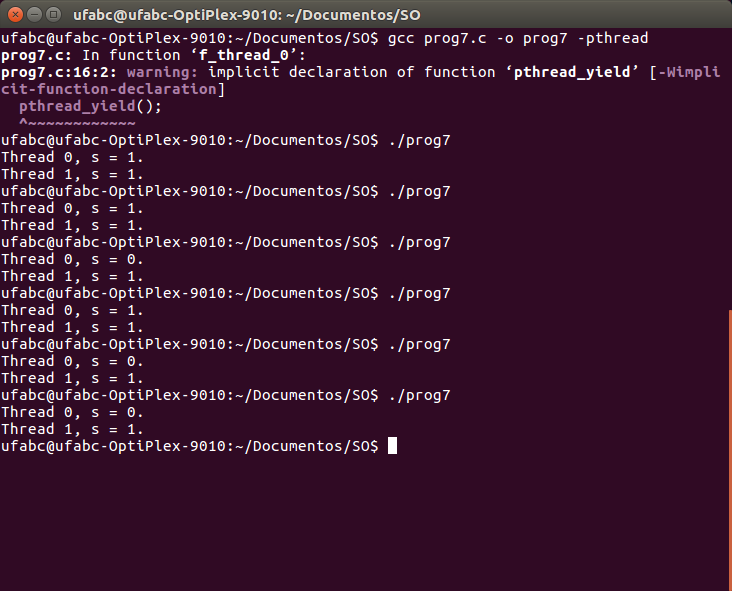
\includegraphics[trim=0 110 0 0,clip,scale=.4]{pratica1/prog7.png}
    \captionof{figure}{Execução do código prog7.c}
    \label{prog4modpng}
    \hspace{1em}
\end{minipage}

\subsection*{6. Implementando a exclusão mútua}
\addcontentsline{toc}{section}{6. Implementando a exclusão mútua}

\subsubsection{6.1 - Compile com a opção -pthread o programa prog8.c. Execute-o várias vezes e comente sobre as saídas.}
\addcontentsline{toc}{subsection}{Exercício 6.1}

\vspace{-0.5em}
\begin{minipage}{\textwidth}
  \hspace{-1em}
  \centering
  \lstinputlisting[language=C]{pratica1/prog8.c}
  \captionof{figure}{Código fonte do programa prog8.c}
  \label{prog4mod}
  \hspace{1em}
\end{minipage}
\vspace{0.5em}

Agora, com a implementação do semáfaro Mutex, cada thread corretamente imprime o valor que atribuiu a variável, pois não há alteração da variável por outras threads enquanto cada thread opera. Note, no entanto, que elas ainda podem imprimir fora de ordem, pois não há como controlar qual thread entrará na região crítica primeiro.

\vspace{2em}
\begin{minipage}{\textwidth}
    \hspace{-1em}
    \centering
    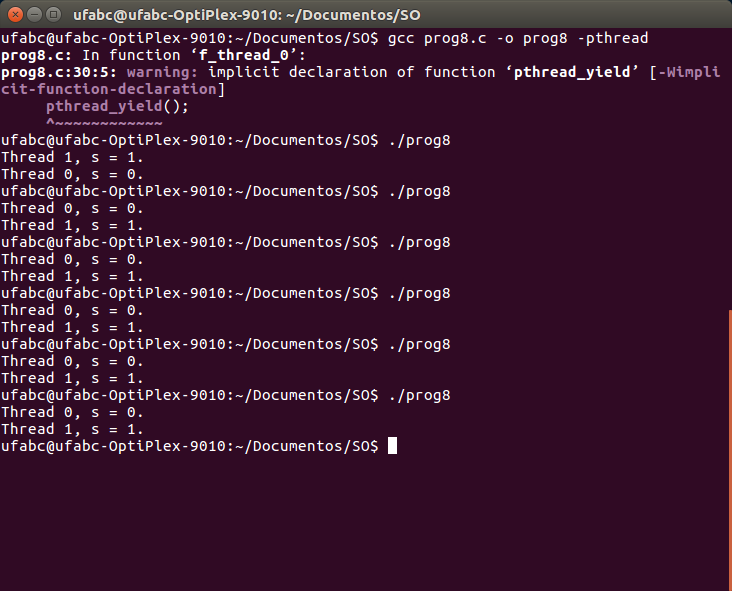
\includegraphics[trim=0 110 0 0,clip,scale=.4]{pratica1/prog8.png}
    \captionof{figure}{Execução do código prog8.c}
    \label{prog4modpng}
    \hspace{1em}
\end{minipage}

\subsection*{7. Produtor-consumidor com troca de mensagens.}
\addcontentsline{toc}{section}{7. Produtor-consumidor com troca de mensagens.}

\subsubsection{7.1 - Compile com a opção -o cons o programa prog9c.c. Compile com a opção -o prod o programa prog9p.c. Execute os programas cons e prod em diversas combinações. Explique o funcionamento dos programas.}
\addcontentsline{toc}{subsection}{Exercício 7.1}

\vspace{-0.5em}
\begin{minipage}{\textwidth}
    \hspace{1em}
    \centering
    \begin{minipage}[t]{0.475\textwidth}
        \centering
        \lstinputlisting[language=C]{pratica1/prog9p.c}
        \label{prog4mod}
    \end{minipage}
    \hfill
    \begin{minipage}[t]{0.475\textwidth}
        \centering
        \lstinputlisting[language=C]{pratica1/prog9c.c}
        \label{prog4mod}
    \end{minipage}
    \hspace{1em}
    \\[-3pt]
    \hspace{1em}
    \begin{minipage}[t]{.475\linewidth}
        \centering
        \captionof{figure}{Código fonte do programa prog9p.c}
    \end{minipage}%
    \hfill%
    \begin{minipage}[t]{.475\linewidth}
        \centering
        \captionof{figure}{Código fonte do programa prog9c.c}
    \end{minipage}%
    \hspace{1em}
\end{minipage}
\vspace{1em}

Ambos os programas solicitam na linha 24 uma mailbox na porta definida na linha 17. O produtor, então, na linha 34 envia a mensagem à mailbox alvo. O consumidor executa, na linha 31, o comando bloqueador de receber mensagem, e consome a primeira mensagem na mailbox ou o processo dorme até que uma mensagem chegue.

\vspace{2em}
\begin{minipage}{\textwidth}
    \hspace{-1em}
    \centering
    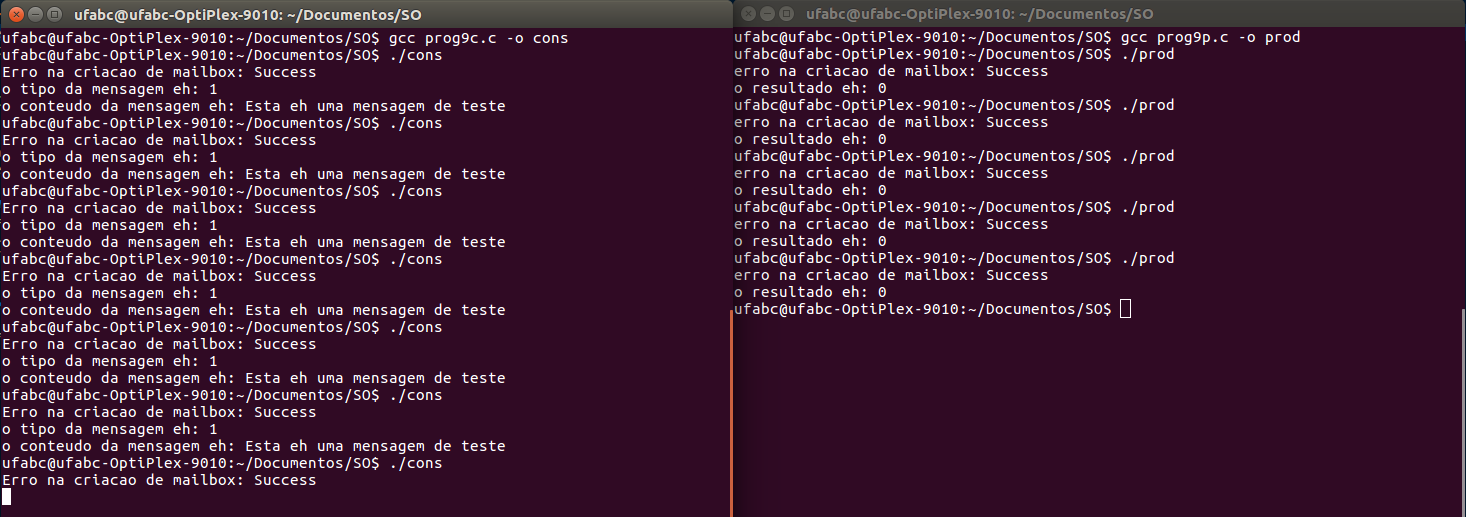
\includegraphics[trim=0 0 0 0,clip,scale=.3]{pratica1/prog9.png}
    \captionof{figure}{Execução do código prog9.c}
    \label{prog4modpng}
    \hspace{1em}
\end{minipage}

\subsubsection{7.2 - Modifique os programas prog9c.c e prog9p.c para implementar o sistema produtor-consumidor com N mensagens da Figura 2.29 do livro texto (Aula 3 - página 30), mas fazendo uso de caixa postal.}
\addcontentsline{toc}{subsection}{Exercício 7.2}

\vspace{-0.5em}
\begin{minipage}{\textwidth}
    \hspace{1em}
    \centering
    \begin{minipage}[t]{0.475\textwidth}
        \centering
        \lstinputlisting[language=C]{pratica1/prog9pmod.c}
        \label{prog4mod}
    \end{minipage}
    \hfill
    \begin{minipage}[t]{0.475\textwidth}
        \centering
        \lstinputlisting[language=C]{pratica1/prog9cmod.c}
        \label{prog4mod}
    \end{minipage}
    \hspace{1em}
    \\[-3pt]
    \hspace{1em}
    \begin{minipage}[t]{.475\linewidth}
        \centering
        \captionof{figure}{Código fonte do programa prog9p.c modificado}
    \end{minipage}%
    \hfill%
    \begin{minipage}[t]{.475\linewidth}
        \centering
        \captionof{figure}{Código fonte do programa prog9c.c modificado}
    \end{minipage}%
    \hspace{1em}
\end{minipage}
\vspace{1em}

Os programas foram testados com BOX{\_}SIZE = 100 e MAX{\_}MSGS = 20000, porém por simplicidade colocamos aqui um exemplo reduzido.

\vspace{2em}
\begin{minipage}{\textwidth}
    \hspace{-1em}
    \centering
    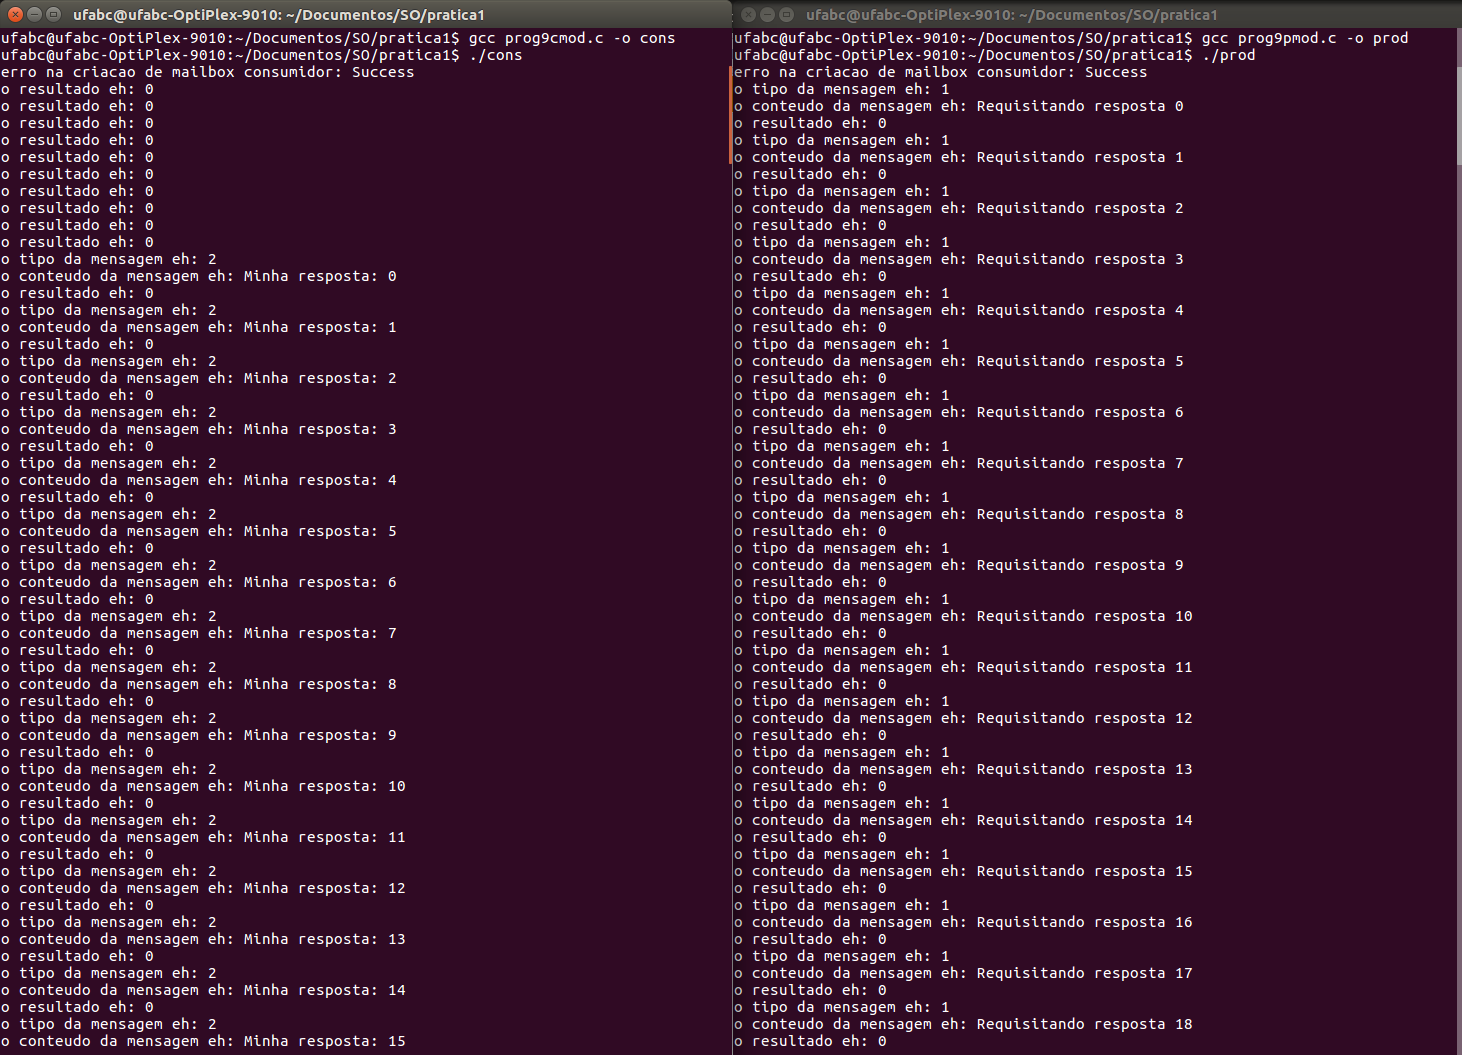
\includegraphics[trim=0 0 0 0,clip,scale=.3]{pratica1/prog9mod.png}
    \captionof{figure}{Início da execução dos programas prog9.c modificados}
    \label{prog4modpng}
    \hspace{1em}
\end{minipage}

\vspace{2em}
\begin{minipage}{\textwidth}
    \hspace{-1em}
    \centering
    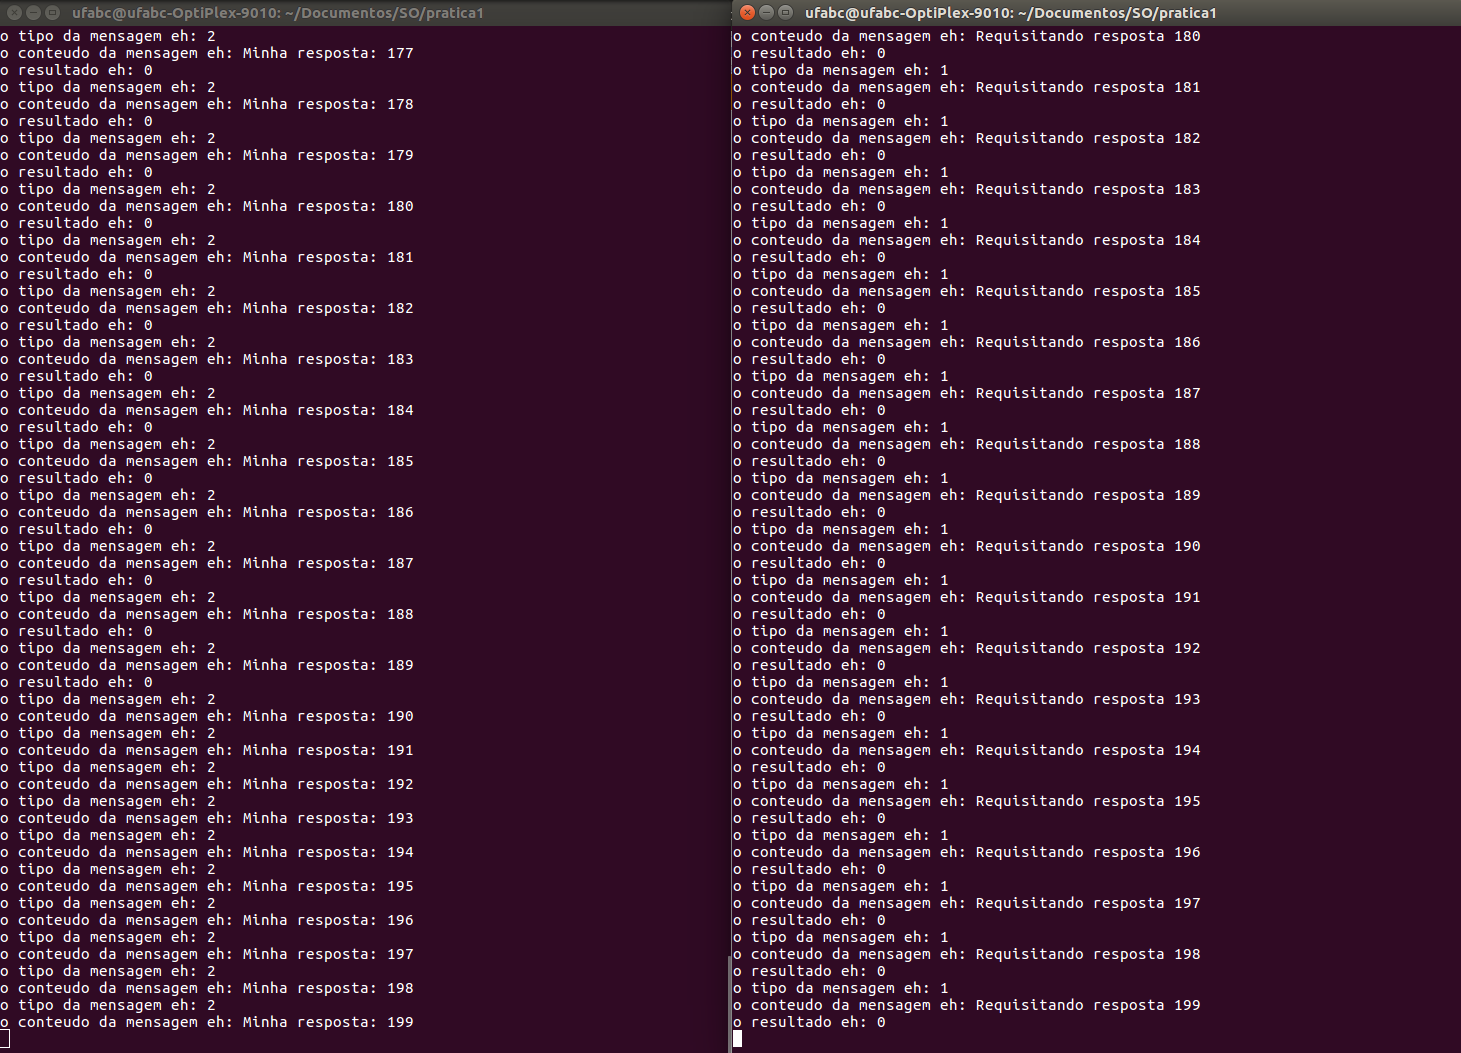
\includegraphics[trim=0 0 0 0,clip,scale=.3]{pratica1/prog9modcont.png}
    \captionof{figure}{Término da execução dos programas prog9.c modificados}
    \label{prog4modpng}
    \hspace{1em}
\end{minipage}